\section*{Exercice 128 -- Statique}
\setcounter{exo}{0}
%POLE JC



On s’intéresse à une console portante de bateau destinée à mettre
les bateaux à l’eau ou à les en retirer à partir d’un quai dans les ports
de plaisance.
Un modèle du mécanisme est représenté ci-dessous. Il est
constitué :
\begin{itemize}
\item  d’un support (0) de repère associé $\rep{0}= \repere{O}{x_0}{y_0}{z_0}$;
\item d’un ensemble 1 (console + câbles + bateau), de repère
associé $\rep{1}= \repere{O}{x_1}{y_1}{z_0}$, de masse maximale $m=\SI{4000}{kg}$ et de centre de gravité $G$ tel que $\vect{OG} = a \vect{x_1} +  b\vect{z_1}$ avec $a =\SI{6}{m}$ et $b =\SI{4}{m}$.
\end{itemize}
La liaison pivot entre 0 et 1 est motorisée.
Les sollicitations proviennent :
\begin{itemize}
\item du poids de l’ensemble 1, force de résultante $-mg \vect{z_0}$ passant par $G$ ;
\item de l’action du vent sur le bateau dans les conditions les plus défavorables $\torseurstat{T}{\text{vent}}{1}$ $=\torseurl{-F_{\text{vent}}\vect{y_1}}{\vect{0}}{G} $ avec $F_{\text{vent}}=\SI{1500}{daN}$;
\item d’un motoréducteur placé entre 0 et 1 exerçant un couple de moment $C_{01}\vect{z_0}$. 
\end{itemize}




\begin{center}
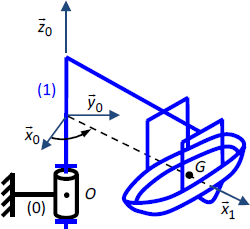
\includegraphics[width=.8\linewidth]{096_02}
\end{center}


\begin{obj}
Afin de dimensionner les constituants qui les réalisent, déterminer les actions transmises par le
vérin et la liaison entre (1) et (0).
\end{obj}

\subparagraph{}\textit{Positionner sur le schéma, à l’aide de vecteurs, les résultantes des actions mécaniques du vérin, du ressort et de la
pesanteur.}
\ifprof
\begin{corrige}
\end{corrrige}
\else
\fi


\subparagraph{}\textit{Réaliser le graphe de structure et la figure de changement de base.}
\ifprof
\begin{corrige}
\end{corrrige}
\else
\fi


\subparagraph{}\textit{Isoler 1 et déterminer, lorsque le mécanisme est à l’équilibre, les 6 équations issues du PFS exprimé en $O$.}
\ifprof
\begin{corrige}
\end{corrrige}
\else
\fi


\subparagraph{}\textit{En déduire les expressions du torseur des actions mécaniques transmises par la liaison entre 1 et 0 et de l’action du motoréducteur.}
\ifprof
\begin{corrige}
\end{corrrige}
\else
\fi


\subparagraph{}\textit{Exprimer le torseur des actions mécaniques transmises par la liaison entre 1 et 0 en fonction de $m$,$g$, $a$, $b$, $k$, $y$ et $y_0$.}
\ifprof
\begin{corrige}
\end{corrrige}
\else
\fi

